\chapter{Oprogramowanie}

W celu wykonania badań, które ocenią możliwości optymalizacji procesu produkcji elektroniki, konieczne było zaimplementowanie odpowiednich algorytmów.
Z względu na to, że Flow Shop jest algorytmem NP-trudny często rezygnuje się z algorytmów dokładnych. Powodem takiego stanu rzeczy jest złożoność obliczeniowa która wynosi $O(n!)$.

W przedstawionym przypadku użyty został algorytm dokładny (przegląd zupełny), ponieważ liczba zadań jest niewielka oraz planowanie w systemie jest offline (nie ma ograniczeń czasowych na uzyskanie rozwiązania).
W celu porównania wybrano algorytm metaheurystyczny (symulowane wyżarzanie), który nie daje rozwiązania optymalnego, lecz dostatecznie dobre w krótkim czasie.

\section{Implementacja}
Program stworzony w celu badań został napisany w języku C++ przy wykorzystaniu środowiska Qt. Jest to zestaw darmowych narzędzi i bibliotek, służących do tworzenia aplikacji okienkowych oraz konsolowych. Niewątpliwą zaletą Qt jest jego wieloplatformowość, dzięki czemu przy użyciu jednego kodu bazowego, może on być zaimplementowany w różnych środowiskach (Windows, Linux, macOS, Android oraz systemy wbudowane).

\breakparagraph{}
W celu łatwego i usystematyzowanego dostępu do informacji o poszczególnych projektach i czasach wykonywania, zaprojektowano i stworzono bazę danych. Zastosowany został system zarządzania bazą danych SQLite.

\breakparagraph{}
Zalety SQLite:
\begin{itemize}
	\item rozwiązanie wieloplatformowe,
	\item cała baza danych to tylko jeden plik,
	\item duża zgodność z standardem SQL,
	\item duża wydajność (silnik napisany w języku C).
\end{itemize}

\newpage{}
\paragraph{}
Projekt bazy danych składa się z trzech tabel (Rysunek~\ref{baza_danych}):
\begin{itemize}
	\item projects --- tabela zawierające podstawowe informacje o poszczególnych projektach,
	\item operation\_time --- tabela zawierająca czasy trwania poszczególnych operacji per projekt,
	\item changeover\_time --- tabela zawierająca czasy przezbrojenia poszczególnych projektów.
\end{itemize}

\begin{figure}[H]
	\centering
	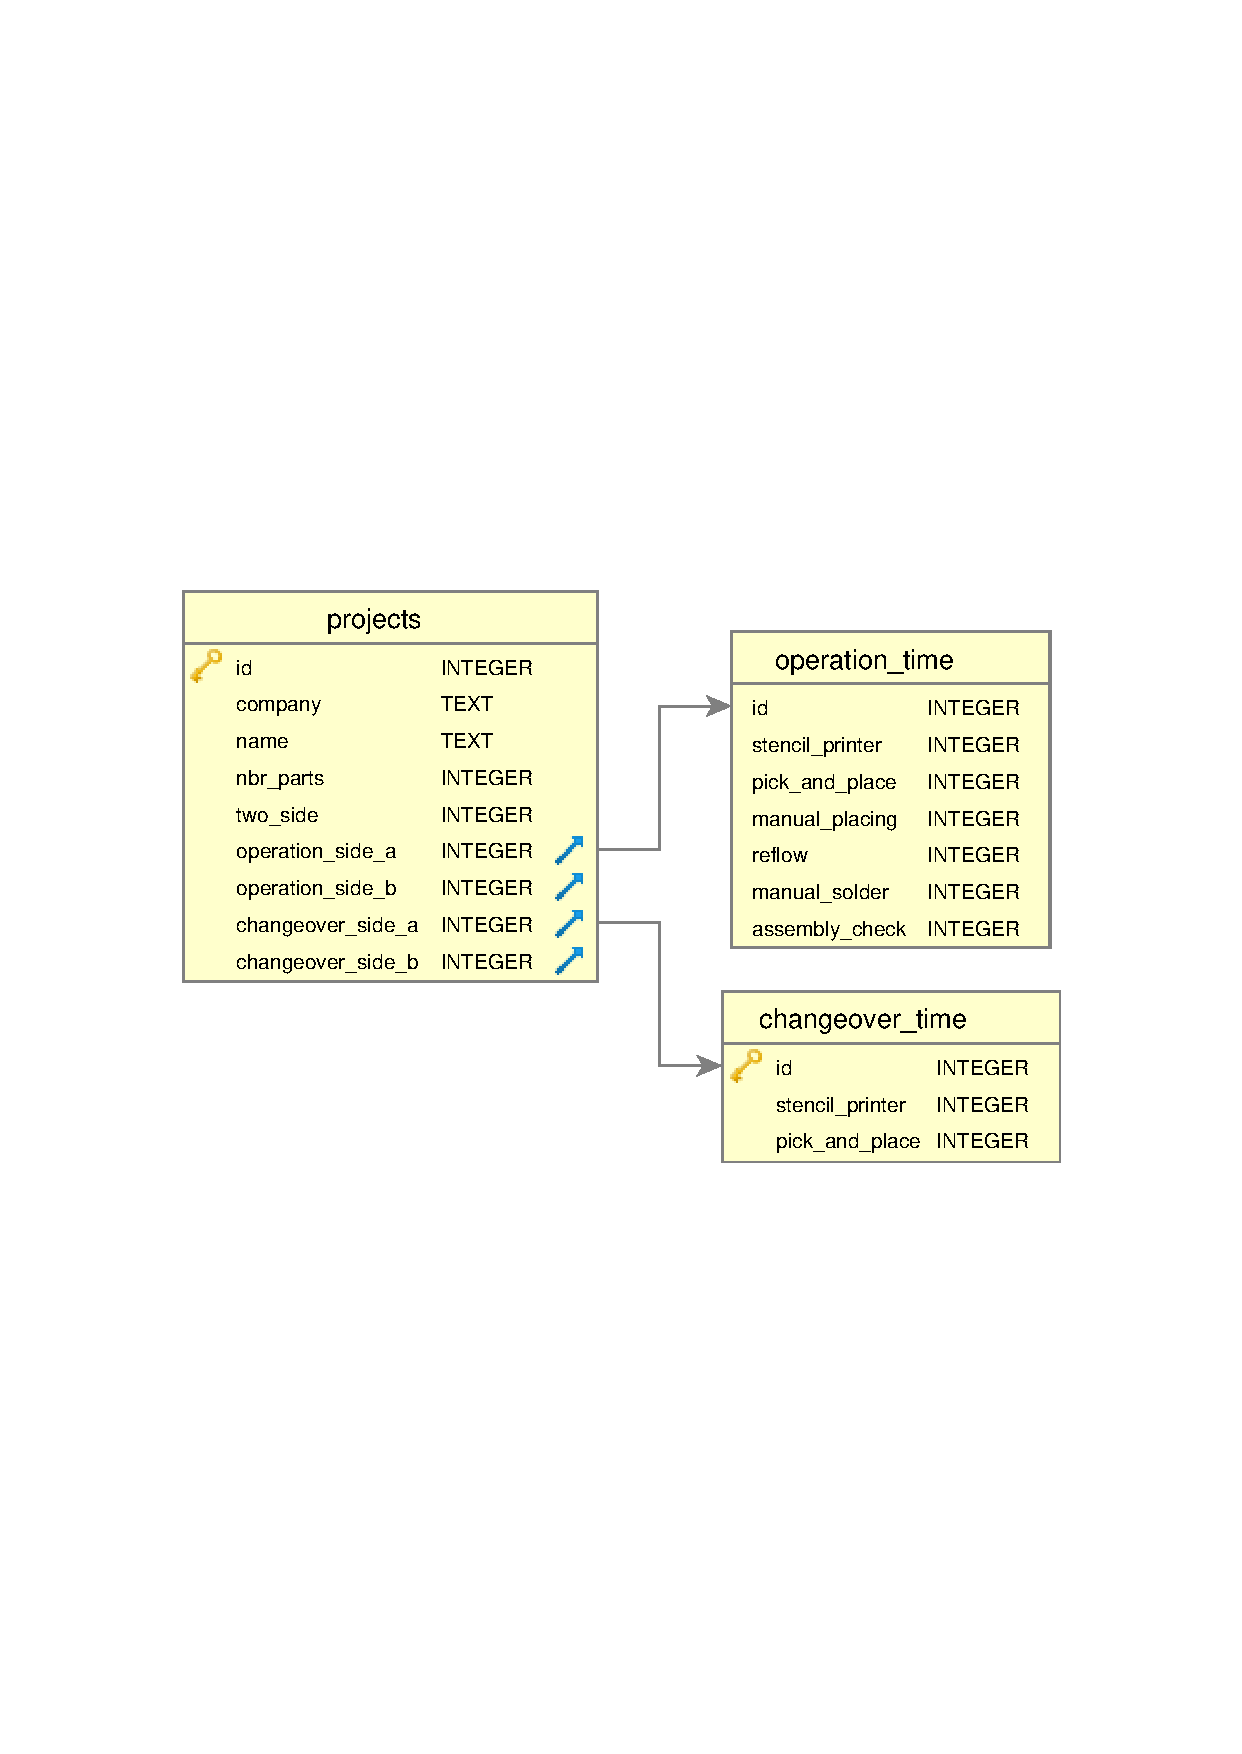
\includegraphics[scale=0.9]{chapters/chapter4/db_crop.pdf}
	\caption{Struktura bazy danych}
	\label{baza_danych}
\end{figure}

\begin{table}[H]
	\centering
	\caption{Opis pól w tabeli ``projects''}
	\begin{tabular}{lll}
		\toprule
		Pole tabeli         & Opis                                    & Format pola       \\
		\midrule
		id                  & Indeks projektu                         & Liczba całkowita \\
		company             & Nazwa firmy                             & Tekst             \\
		name                & Nazwa projektu                          & Tekst             \\
		nbr\_parts          & Ilość elementów                      & Liczba całkowita \\
		two\_side           & Czy płyta posiada 2 warstwy            & Liczba całkowita \\
		operation\_side\_a  & Indeks do czasów operacji dla strony A & Liczba całkowita \\
		operation\_side\_b  & Indeks do czasów operacji dla strony B & Liczba całkowita \\
		changeover\_side\_a & Indeks do czasów przezbrojenia         & Liczba całkowita \\
		changeover\_side\_b & Indeks do czasów przezbrojenia         & Liczba całkowita \\
		\bottomrule
	\end{tabular}
\end{table}

\begin{table}[H]
	\centering
	\caption{Opis pól w tabeli ``changeover\_time''}
	\begin{tabular}{lll}
		\toprule
		Pole tabeli      & Opis                              & Format pola       \\
		\midrule
		id               & Indeks rekordu                    & Liczba całkowita \\
		stencil\_printer & Czas przezbrojenia na sitodruku   & Liczba całkowita \\
		pick\_and\_place & Czas przezbrojenia na pick\&place & Liczba całkowita \\
		\bottomrule
	\end{tabular}
\end{table}

\begin{table}[H]
	\centering
	\caption{Opis pól w tabeli ``operation\_time''}
	\begin{tabular}{lll}
		\toprule
		Pole tabeli      & Opis                                          & Format pola       \\
		\midrule
		id               & Indeks rekordu                                & Liczba całkowita \\
		stencil\_printer & Czas operacji na sitodruku                    & Liczba całkowita \\
		pick\_and\_place & Czas operacji na pick\&place                  & Liczba całkowita \\
		manual\_placing  & Czas operacji ręcznego nakładani elementów & Liczba całkowita \\
		reflow           & Czas operacji lutowania w piecu               & Liczba całkowita \\
		manual\_solder   & Czas operacji ręcznego lutowania             & Liczba całkowita \\
		assembly\_check  & Czas operacji kontroli wizualnej              & Liczba całkowita \\

		\bottomrule
	\end{tabular}
\end{table}

\newpage{}
\section{Przegląd zupełny}

Przegląd zupełny (ang. Brute-force search) jest to algorytm polegający na wyznaczeniu wszystkich możliwych permutacji zadania, a następnie wybraniu z tego zbioru rozwiązania najlepszego. Jest to algorytm dokładny, przez co rozwiązanie jest zawsze optymalne, lecz niestety okupione dużą złożonością.

Diagram na Rysuneku~\ref{brute_force} przedstawia ideę algorytmu. W celu wygenerowania wszystkich permutacji zadań wykorzystano algorytm porządku leksykograficznego (Rysunek~\ref{gen_perm}).

\section{Symulowane wyżarzanie}
Symulowane wyżarzanie (ang. Simulated annealing, SA) to kombinatoryczna metoda optymalizacji oparta na szukaniu losowo rozwiązania~\cite{sa}. Algorytm ten oparty jest na analogii pomiędzy zjawiskiem wyżarzania metali, a optymalizacją złożonych problemów kombinatorycznych. Wiele tych problemów jest NP-trudnych, co powoduje, że istnienie algorytmów dokładnych, o wielomianowym czasie obliczeniowym, jest niemożliwe. Symulowane wyżarzanie jest zatem idealnym wyborem ze względu na jego elastyczność, szybkość działania oraz jakość rozwiązań, przez co nie ma ograniczeń przy doborze do problemu.

Głównym parametrem w badanym algorytmie jest temperatura. To ona odpowiada za to, jak intensywny będzie ruch cząsteczek. Duża ruchliwość cząsteczek umożliwia szersze przeszukanie przestrzeni rozwiązań. Dzięki temu minimalizujemy szanse na utknięcie algorytmu w minimum lokalnym podczas optymalizacji. Wraz z postępowaniem symulowanego wyżarzania, temperatura jest zmniejszana.

W algorytmie SA istotną rolę odgrywają: dobór odpowiednich parametrów, strategii schładzania oraz dobranie techniki ruchu po przestrzeni.

\breakparagraph{}
Symulowane wyżarzanie posiada 3 parametry wpływające na jego działanie:
\begin{itemize}
	\item $T_{start}$ --- temperatura początkowa (wartość początkowa temperatury),
	\item $T_{stop}$ --- temperatura końcowa (warunek stopu),
	\item $\lambda$ --- współczynnik schładzania (tempo, w jakim temperatura ma spadać).
\end{itemize}

\breakparagraph{}
Stosuję się najczęściej dwa schematy schładzania~\cite{Smutnicki2002As}:
\begin{itemize}
	\item geometryczny $T = \lambda T$
	\item logarytmiczny $T = T /(1 + \lambda T)$
\end{itemize}

Wybór strategii schładzania zależy w dużej mierze od problemu jaki, został postawiony przed algorytmem.

\breakparagraph{}
W pracy zaimplementowano podstawową wersję algorytmu (Rysunek~\ref{sa}).
\raggedbottom{}


\section{Diagramy}
\begin{figure}[H]
	\centering
	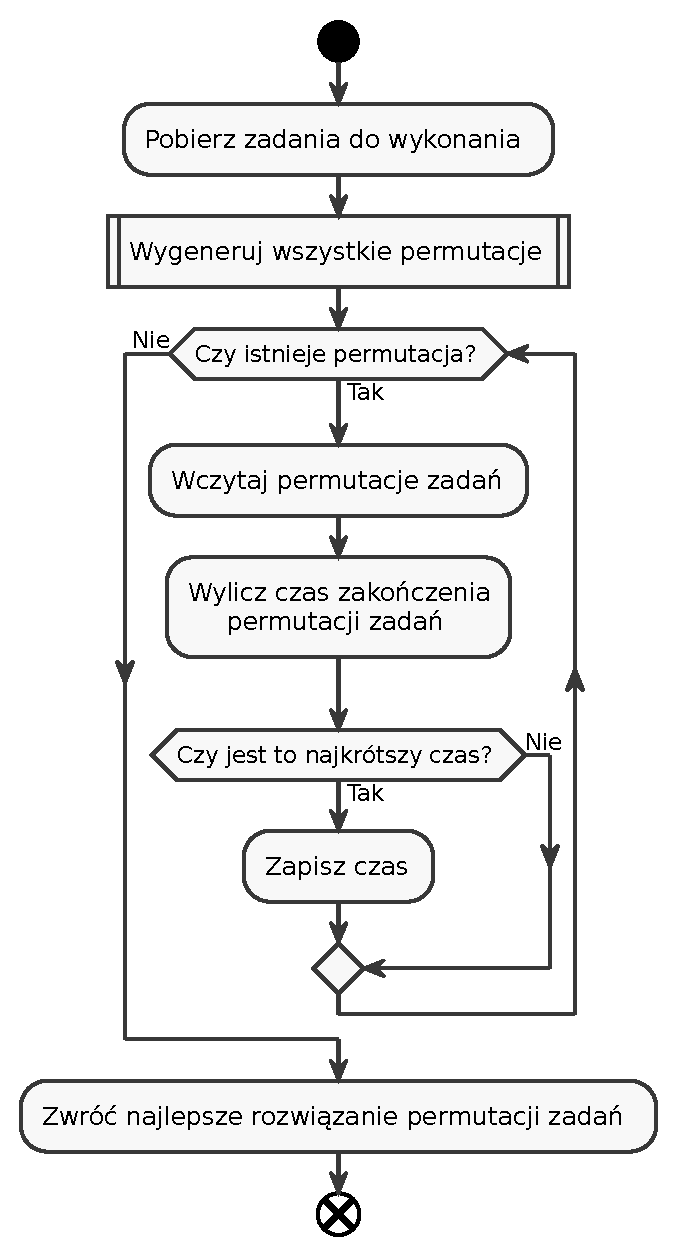
\includegraphics[]{chapters/chapter4/brute_force.pdf}
	\caption{Diagram algorytmu ``Przegląd zupełny''}
	\label{brute_force}
\end{figure}

\begin{figure}[H]
	\centering
	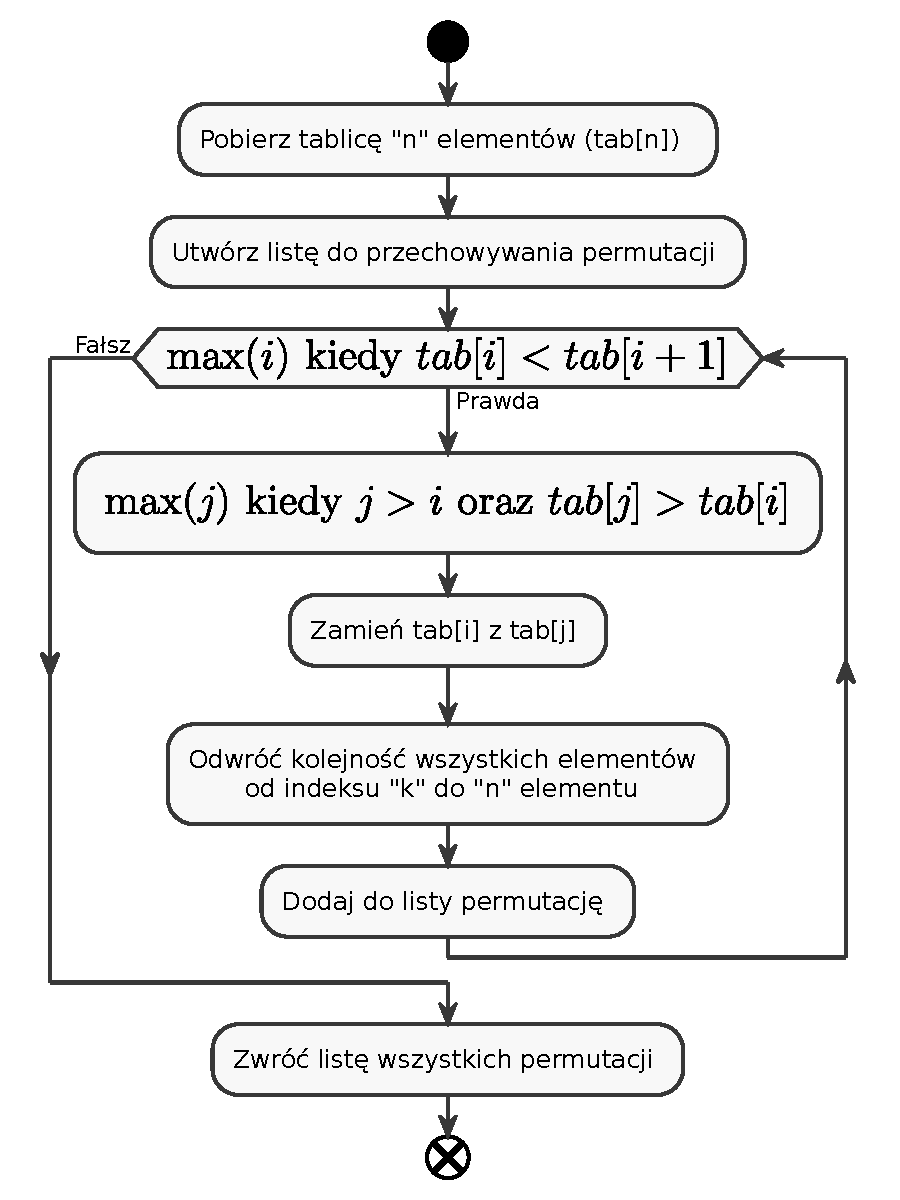
\includegraphics[]{chapters/chapter4/gen_perm.pdf}
	\caption{Diagram algorytmu ``Porządek leksykograficzny''}
	\label{gen_perm}
\end{figure}



\begin{figure}[H]
	\centering
	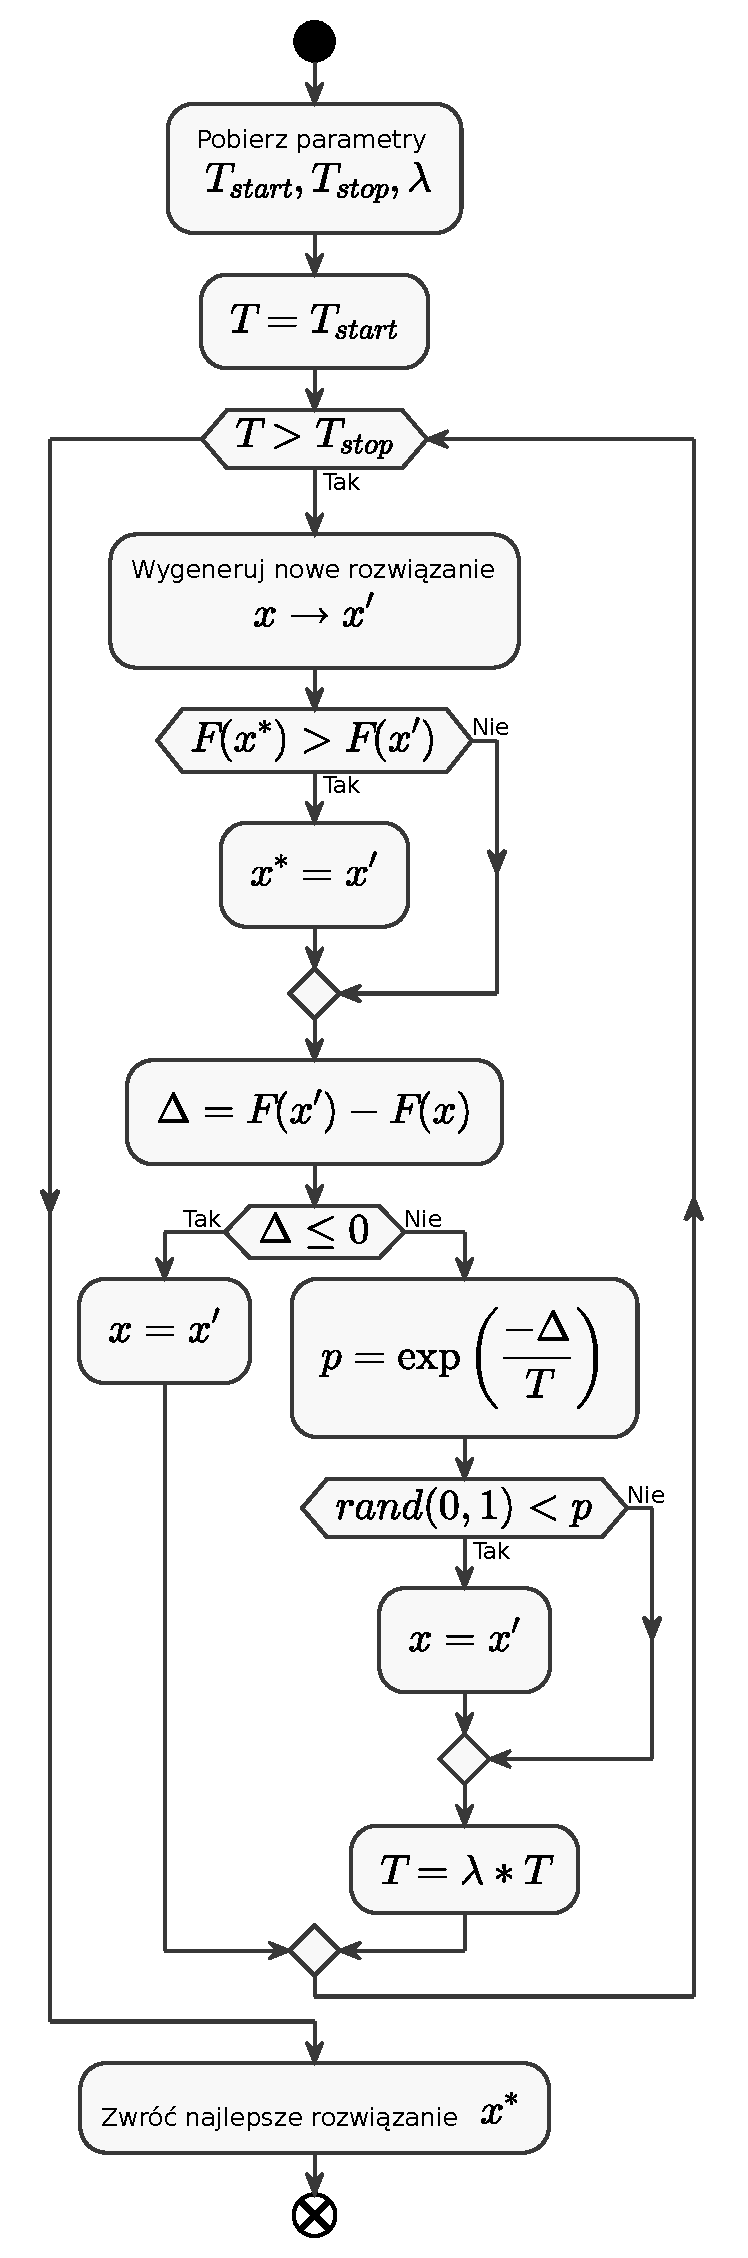
\includegraphics[scale=0.67]{chapters/chapter4/sa.pdf}
	\caption{Diagram algorytmu ``Symulowane wyżarzanie''}
	\label{sa}
\end{figure}
